%用来打印中文
\documentclass[UTF8]{ctexart}
\RequirePackage{iftex}
\RequirePackage{fix-cm}
\RequirePackage{fixltx2e}
%页面设置
\RequirePackage{geometry}
\if@twoside
 \geometry{a4paper,
 bindingoffset = 2cm,
 inner = 0.5cm,
 outer = 2cm,
 top = 3cm,
 bottom = 2cm
 }
\else
 \geometry{a4paper,
 left = 2cm,
 right = 2cm,
 top = 2cm,
 bottom = 2cm
 }
%各种包
\usepackage{fancyhdr}
\usepackage{amssymb}
\RequirePackage{graphicx}
\RequirePackage{subfigure}
\RequirePackage{caption}
\RequirePackage{diagbox}
\RequirePackage{multirow}
\RequirePackage{makecell}
\RequirePackage{booktabs}
%\usepackage{lipsum}
\usepackage{mathtools}
\usepackage{listings}%代码
%矩阵
\usepackage{amsmath,xcolor}
\RequirePackage{longtable}
\RequirePackage{array}
%页眉
\RequirePackage{float}
\RequirePackage{flowchart}
\pagestyle{fancy}
\renewcommand{\headrulewidth}{0.5pt} 
\lhead{} \rhead{name\ number}%\thepage
% 顶格写\noindent
\begin{document}
%\pagenumbering{arabic}
\section*{Discrete Mathematics Homework-7}
\begin{center}
\today
\end{center}
\subsection*{Assignment}

Page 155 \ 29\ 30
\\

Page 188 \ 4\ 7(2)\ 9\ 13

\subsection*{•29设A是集合,不使用无序对集合存在公理证明\{A\}是集合}

由空集合存在公理知,存在集合$\emptyset$

由幂集合公理,对于任意集合x,存在一个集合y,其元素恰好为x的子集,即集合的幂集是集合,则存在集合$\{\emptyset\}$,设为t。

定义谓词$P(x,y)$为$P(\emptyset ,A)=T$,则t、P(x,y)满足替换公理模式前提,则$s=\{A\}$是集合,得证。


\subsection*{•30证明不存在集合$A_1$,$A_2$,$A_3$,$A_4$使$A_4\in A_3\wedge A_3\in A_2\wedge A_2\in A_1\wedge A_1\in A_4 $.}

假设存在集合使得$A_1$,$A_2$,$A_3$,$A_4$使$A_4\in A_3\wedge A_3\in A_2\wedge A_2\in A_1\wedge A_1\in A_4 $.

由无序对集合存在公理$\{A_1,A_2\}$、$\{A_3,A_4\}$、$\{\{A_1,A_2\},\{A_3,A_4\}\}$是集合.

由并集公理得对于集合$\{\{A_1,A_2\},\{A_3,A_4\}\}$,存在集合$B=\{A_1,A_2,A_3,A_4\}$.

由$A_4\in A_3$,$A_4\in B$得$A_4\in A_3\cap B$,即$A_3\cap B\neq \emptyset$,同理$A_2\cap B\neq \emptyset$、$A_1\cap B\neq \emptyset$、$A_4\cap B\neq \emptyset$.该结论与正则公理矛盾,则假设不成立.不存在集合$A_1$,$A_2$,$A_3$,$A_4$使$A_4\in A_3\wedge A_3\in A_2\wedge A_2\in A_1\wedge A_1\in A_4 $.证毕.

\subsection*{•4设A=\{1,2,3\},在A上有多少不同的关系?设$\mid A\mid =n$,在A上有对少不同的关系?}

$3^2=9\quad 2^9=512$

$2^{n^2}$
\subsection*{•7(2)对A=\{0,1,2,3,4\}上的关系$R_2=\{<x,y>\mid 0\leqslant (x-y)\leqslant 3 \}$,给出关系图和关系矩阵}

关系图:
\begin{figure}[H]
  \centering
  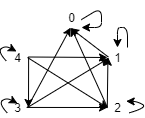
\includegraphics[totalheight=2in]{HW7_4.png}
  \caption{关系图} \label{fig:graph}
\end{figure}

关系矩阵:

\begin{displaymath}
M(R_2)= \left[
\begin{matrix}
   1 & 0 & 0 &0 &0\\
   1 & 1 & 0 &0 &0\\
   1 & 1 & 1 &0 &0\\
   1 & 1 & 1 &1 &0\\
   0 & 1 & 1 &1 &1\\
\end{matrix}
\right] 
\end{displaymath}

\subsection*{•9\ $A=\{<\emptyset ,\{\emptyset , \{\emptyset\}\} >,<\{\emptyset \},\emptyset > \}$,写出}

\subsubsection*{$A\circ A =\{<\{\emptyset \},\{\emptyset , \{\emptyset\}\}>\}$}
\subsubsection*{$A^{-1}=\{<\{\emptyset , \{\emptyset\}\},\emptyset >,<\emptyset ,\{\emptyset \} > \} $}
\subsubsection*{$A\upharpoonright \emptyset =\emptyset $}
\subsubsection*{$A\upharpoonright \{\emptyset\}=<\emptyset ,\{\emptyset , \{\emptyset\}\} > $}
\subsubsection*{$A\upharpoonright \{\emptyset ,\{\emptyset\}\}=A $}
\subsubsection*{$A[\emptyset ] = \emptyset $}
\subsubsection*{$A[\{\emptyset\}]= \{\{\emptyset , \{\emptyset\}\} \}$}
\subsubsection*{$A[\{\emptyset ,\{\emptyset\}\}] =\{\{\emptyset , \{\emptyset\}\},\emptyset \}$}
\subsection*{•13对A到B的关系R,$a\in A$,定义B的一个子集$R(a)=\{b\mid aRb\}$.\\在C=\{-4,-3,-2,-1,0,1,2,3,4\}上定义$R=\{<x,y>\mid x<y\},S=\{<x,y>\mid x-1<y<x+2\},T=\{<x,y>\mid x^2\leqslant y\}$.写出集合R(0),R(1),S(0),S(-1),T(0),T(-1).}

R(0)=$\{1,2,3,4\} $

R(1)=$\{2,3,4\} $

S(0)=$\{0,1\} $

S(-1)=$\{-1,0\} $

T(0)=$\{0,1,2,3,4\} $

T(-1)= $\{1,2,3,4\} $

\end{document}
